\documentclass[a4paper,10pt]{article}

\usepackage[utf8]{inputenc}
\usepackage{t1enc}

\usepackage[utf8]{inputenc}
\usepackage{t1enc}
\usepackage[spanish]{babel}
\usepackage[pdftex,usenames,dvipsnames]{color}
\usepackage[pdftex]{graphicx}
\usepackage{enumerate}
\usepackage{amsmath}
\usepackage{amsfonts}
\usepackage{amssymb}
\usepackage[table]{xcolor}
\usepackage[small,bf]{caption}
\usepackage{float}
\usepackage{subfig}
\usepackage{listings}
\usepackage{bm}
\usepackage{times}
\usepackage{verbatim}
\usepackage{moreverb}
\usepackage{fancyvrb}
% \usepackage{hyperref}
\usepackage{multirow}
\usepackage{url}
\usepackage{listings}
\lstset{breaklines=true}
\lstset{numbers=left, numberstyle=\scriptsize\ttfamily, numbersep=10pt, captionpos=b} 
\lstset{basicstyle=\small\ttfamily}
\lstset{framesep=4pt}

\begin{document}
\setcounter{secnumdepth}{5}
\setcounter{tocdepth}{5}

\begin{titlepage}
        \vfill
        \thispagestyle{empty}
        \begin{center}
                
\includegraphics{./images/itba_logo.png}
                \vfill
                \Huge{Criptografia y Seguridad}\\
                \vspace{1cm}
                \Huge{Esteganografía}\\
                \vspace{1cm}
                \Huge{Trabajo Pr\'actico Especial 2}\\
        \end{center}
        \vfill
        \large{
        \begin{tabular}{lcr}
                Civile, Juan Pablo && 50453\\
                Crespo, Alvaro && 50758 \\
                Susnisky, Dario && 50592\\
        \end{tabular}
}
        \vspace{2cm}
        \begin{center}
                \large{10 de Junio de 2013}\\
        \end{center}
\end{titlepage}
\newpage

\setcounter{page}{1}

\section{Introducción}

En el presente Trabajo Práctico se muestan los resultados y análisis generados a partir del programa \textit{stegobmp}, implementado según la especificación
brindada por la cátedra. Dicho programa brinda la posibilidad de ocultar un archivo cualquiera en un archivo \textit{bmp}, mediante un método de estenografiado específico, 
con la posibilidad de encriptarlo. De igual forma, el programa permite recuperar el archivo oculto a partir de un archivo \textit{bmp}, que haya sido estenografiado con alguno 
de los métodos provistos.\\

Se presentan los resultados obtenidos a partir de las imágenes provistas por la cátedra, junto con el análisis de los mismos.
También se incluye el análisis de algunas cuestiones interesantes, establecidas por la cátedra.

\section{Desarrollo}

\subsection{Estegoanálisis de los archivos provistos}

El desarrollo detallado del proceso de stegoanálisis de los archivos provistos por la cátedra se puede encontrar en la respuesta de la pregunta 5 de la siguiente sección.
Allí se halla explicitado el procedimiento completo para extraer cada uno de los mensajes ocultos y los pasos que se debieron realizar.\\

\subsection{Cuestiones a analizar}

\subsubsection*{ 1) Para la implementación del programa \textit{stegobmp} se pide que la ocultación comience en el
primer componente del primer pixel. ¿Sería mejor empezar en otra ubicación? ¿Por qué?}

Dado que la ocultación que se utiliza se basa en el método LSB (\textit{\textbf{Least Significant Bit}}), los bits ``aprovechables'' son pocos. En el caso de 
LSB1, se pueden utilizar 1 de cada 8 bits, (el bit menos significativo de cada byte). Si se usa LSB4, se pueden utilizar 4 de cada 8, lo que mejor bastante la cantidad de 
espacio ``aprovechable''. Aún así, utilizando los últimos 4 bits de cada byte, ya se está introduciendo una disposición no menor, por lo que la cuestión del espacio resulta 
importante. \\

Por lo tanto, es conveniente empezar la ocultación desde el comienzo de la imagen, es decir el primer pixel, para poder disponer de toda la imagen para, en caso de ser necesario,
ocultar en los bits menos significativos, la información del mensaje oculto.\\

Otra cuestión de interés, es que si se oculta información siempre en los bits menos significativos en orden, es más fácil localizar y extraer la información oculta, podría 
ser mejor solo ocultar en los bits menos significativos de una secuencia aleatoria basada en una clave o algo similar. De está forma, el lugar donde se comienza la ocultación
pierde su significado, ya que no importa por donde se comienza la ocultación, siempre y cuando se utilice todo el archivo para ocultar.\\

Otro aspecto importante a la hora de escoger el lugar de la imagen es el ruido, es decir, las zonas donde la imagen contiene ruido. Varios autores aseguran, y con razón, que lo mejor 
para minimizar la distorsión de la imagen al ocultar el mensaje, es ocultar el mensaje en las zonas más ruidosas de la imagen, ya que la distorsión atrae menos la atención. Para 
encontrar estas zonas, se utilizan filtros de selección de píxeles.

\subsubsection*{ 2) ¿Qué ventajas podría tener ocultar siempre en una misma componente? Por ejemplo, siempre
en el bit menos significativo de la componente azul.}

Es algo parecido a lo que se propone en el paper Enhanced Least Significant Bit algorithm For Image Steganography de 
Shilpa Gupta, Geeta Gujral y Neha Aggarwal. Se propone el “Enhanced Least Significant Bit (ELSB)”, que consiste justamente en ocultar siempre en 
la primer componente, es decir, en el bit menos significativo de la componente azul.\\

Las ventajas son las obvias. Se distorsiona menos la imagen, ya que solo se altera la banda de los azules. El salto de color es menor, ya que si, por ejemplo se 
cambiará la componente roja, el rango de colores que se saltea es mayor. Recordar que el color se define como la concatenación de 3 valores de 0 a 255, rojo, verde y azul, en 
ese orden, por lo que valor del color azul es menos significativo que los otros dos.\\

La desventaja es también clara: se requiere mayor tamaño de la imagen portadora. Para contrarrestar esto se podría hacer la modificación de solo
cambiar el bit menos significativo, sino 2, 3 o 4, que igualmente generarían una menor distorsión y requieren menor tamaño. De hecho con usar 3 bits se requiere el mismo 
tamaño que al usar LSB-1, lo cual tiene sentido, es lo mismo, en términos de cantidades, tomar 1 bit de cada componente que 
tomar 3 de una sola componente.\\

\subsubsection*{ 3) Esteganografiar un mismo archivo en un .bmp con cada uno de los tres algoritmos, y comparar
los resultados obtenidos. Hacer un cuadro comparativo de los tres algoritmos estableciendo ventajas y desventajas.}

En el Anexo se encuentran las imágenes (figuras \ref{fig:awesome_image3} y \ref{fig:awesome_image4}) luego de haber esteganografiado una misma imagen (figura \ref{fig:awesome_image1}) 
para ocultar una determinada imagen (figura \ref{fig:awesome_image2})
con los algoritmos LSB. Cabe destacar, que con LSBE no se pudo ocultar la imagen deseada porque la imagen portadora solo podía ocultar 22 bytes utilizando ese algoritmo. Esto se debe a que no hay muchos píxeles cuyos valores de alguna 
componente sea 254 o 255.\\

No es fácilmente apreciable, pero puede notarse como, la imagen esteganografiada con LSB4 presenta un poco de distorsión, mientras que la que fue esteganografiada con LSB1 es, a simple
vista, idéntica a la original.\\

El siguiente cuadro refleja la comparación entre los algoritmos de esteganografiado estudiados.\\

\begin{tabular}[\baselineskip]{|l|c|c|c}
    \hline
    Algoritmo & Ventajas & Desventajas \\
    \hline
    LSB-1 &  Menos distorsión & Requiere mayor tamaño del portador \\
    \hline
    LSB-4       & Reduce tamaño requerido       & Más distorsión \\
                &  del portadora                & \\
    \hline
    LSB Enhanced & Mínima distorsión    & Muchísimo tamaño del portador.\\
                 &                      & No hay una relación directa entre \\
                 &                      & el tamaño del portador y del mensaje.\\
    \hline
\end{tabular} 


\subsubsection*{ 4) Para la implementación del programa \textit{stegobmp} se pide que la extensión del archivo se oculte
después del contenido completo del archivo. ¿por qué no conviene ponerla al comienzo, después del tamaño de archivo?}

Podría argumentarse que esteganografiar la extensión por separado no es necesario. Pero lo cierto es que se necesita para rearmar el archivo rápidamente, y sin dejar librado
al usuario del programa que deba adivinar o saber el formato del archivo oculto. Por que si bien el contenido entero podría ocultarse y recuperarse exitosamente, sin la extensión
no se podría nombrar correctamente el archivo, y los sistemas operativos no sabrían con que programas abrirlos. Por otro lado, es cierto que no es una buena idea que 
un atacante pueda, descubriendo una secuencia de unos pocos bits que forman 4 chars identificables, tener mucha información respecto del archivo que se encuentra oculto.
Es por esto que quizás, no sea conveniente poner la extensión al principio, donde puede ser más fácilmente encontrada. De todas formas, esto es discutible, ya que si un atacante logra
descifrar los 4 bytes que determinan el tamaño del archivo, podría encontrar con fácilidad donde se encuentran los caracteres de la extensión, siempre y cuando no se utilice algunas
forma de randomización o alteración del orden de los bits ocultados, como con el uso de una clave.\\

\subsubsection*{ 5) Explicar detalladamente el procedimiento realizado para descubrir qué se había ocultado en
cada archivo y de qué modo.}

Las imágenes aquí referenciadas se encuentran en la sección Anexo.\\

En un principio, se intentó extraer cada archivo con todos los algoritmos de estenografiado, para ver a qué algoritmo respondía cada uno. De esta forma, se 
encontró que el archivo \textit{miserables2.bmp} (figura \ref{fig:awesome_image6}) había sido estenografiado con el algoritmo LSB1, y el mensaje oculto era un archivo \textit{.png}, el cual contenía una 
imagen de un tablero del juego \textit{buscaminas}, a medio terminar (figura \ref{fig:awesome_image9}). En segundo lugar, se encontró que el archivo 
\textit{medianocheparis1.bmp} (figura \ref{fig:awesome_image7}) había sido estenografiado 
con el algoritmo LSB4, y el mensaje oculto era una archivo \textit{.wmv}, pero no se podía reproducir correctamente con ningún reproductor de vídeo, 
tanto en Linux como en Windows como en Mac.
Dejando ese llamativo descubrimiento de lado por un momento, se extrajo satisfactoriamente el archivo \textit{.pdf} del archivo \textit{loimposible.bmp}, el cual conteía el texto
``La password es bienvenido'' (figura \ref{fig:awesome_image10}). Esta imagen había sido esteganografiada con el método LSBE.\\
Luego, se procedió a analizar el cuarto archivo, \textit{secretodesusojos1.bmp} (figura \ref{fig:awesome_image5}), y trás un largo análisis, se descubrió, via un editor hexadecimal, 
que hacia el final del archivo, en la representación en caracteres ASCII, se podía leer el siguiente mensaje: \\

\begin{center}
\textbf{\textit{    ``al .png cambiar extension por .zip y descomprimir.''}}
\end{center}

Ante esta revelación, se siguieron dichas instrucciones, y lo que se obtuvo fue un pequeño archivo de texto, \textit{sol8.txt}, que contenía lo siguiente:

\begin{center}
\textbf{\textit{
    ``cada mina es un 1.\\
    cada fila forma una letra.\\
    Los ascii de las letras empiezan todos en 01.\\
    Asi encontraras el algoritmo que tiene clave de 128 bits y el modo\\
    La password esta en otro archivo\\
    Con algoritmo, modo y password hay un .wmv encriptado y oculto.''
}}
\end{center}

Con este nuevo descubrimiento, se resolvió el mensaje encodeado en la imagen \textit{.png}. \textit{\textbf{Resolviendo}} el tablero del buscaminas, se obtuvo el siguiente resultado:
\begin{center}
\begin{tabular}{|l|c|c|c|}
    \hline
    Binario       & Decimal       & Hexadecimal   & ASCII \\
    \hline
    0100001       & 101           & 41            & A     \\
    \hline
    01100101      & 101           & 65            & e     \\
    \hline
    01110011      & 115           & 73 hex        & s     \\
    \hline
    01000011      & 67            & 43 hex        & C     \\
    \hline
    01100000      & 98            & 62 hex        & b     \\
    \hline
    01100011      & 99            & 63 hex        & c     \\
    \hline
\end{tabular}
\end{center}

Al romper este código, la respuesta era clara, se debía usar el programa \textit{stegobmp} para extraer correctamente el archivo \textit{.wmv}, con el algoritmo de encriptación
\textit{\textbf{aes128}}, en modo \textit{\textbf{cbc}} y utilizando como contraseña \textit{\textbf{bienvenido}}.\\

Finalmente, al realizar la extracción con desencriptación del archivo \textit{medianocheparis1.bmp}, el que había respondido al algoritmo LSB4 y había arrojado un 
\textit{.wmv} corrupto, se obtuvo el archivo \textit{.wmv} deseado. El video mostraba una escena de la película \textit{\textbf{Wanted}} (\textit{\textbf{Se busca}} en castellano)
la cuál habla de una mística máquina de telar, que produce unas telas que tienen un código secreto, según la disposición de los hilos, que establece objectivos para una selecta
comunidad secreta de asesinos.

\subsubsection*{ 6) ¿Qué se encontró en cada archivo?}

Como se dijo en la respuesta anterior, estos son los resultados para cada archivo:

\begin{center}
\begin{tabular}{|l|c|c|}
    \hline
    Archivo portador (BMP)  & Alg. esteganografiado         & Mensaje oculto     \\
    \hline
    miserables2             & LSB1                          & Imagen PNG(archivo ZIP c/ archivo de texto)\\
    \hline
    medianocheparis1        & LSB4 + aes-128-cbc            & Video WMV \\
    \hline
    loimposible             & LSBE                          & Documento PDF\\
    \hline
    secretodesusojos1       & Misterioso                    & Texto (pista para desencriptar el WMV)\\
    \hline
\end{tabular}
\end{center}

\subsubsection*{ 7) Algunos mensajes ocultos tenían, a su vez, otros mensajes ocultos. Indica cuál era ese mensaje
y cómo se había ocultado.}

El mensaje oculto que consistía en una imagen \textit{.png}, era a su vez, un archivo portador de otro mensaje oculto, y además en la imagen se encontraba
un código que, descifrado, proporcionaba el algoritmo y el modo de encriptación para poder extraer correctamente otro de los mensajes ocultos. \\

Para empezar, al archivo se le podía cambiar la extensión a \textit{.zip}, y descomprimirlo, obteniendo un pequeño archivo de texto que contenía instrucciones a seguir.
Algunas de esas instrucciones decían también, que la imagen contenía otro mensaje oculto, el algoritmo y el modo de encriptación para lograr extraer el otro de los mensajes ocultos.
La imagen consistía en un tablero del juego \textit{Buscaminas}, y si se completaba y se seguían las instrucciones para su decodificación, se podía extraer este otro mensaje oculto.
En este caso era \textit{\textbf{aes}} y \textit{\textbf{cbc}}.

\subsubsection*{ 8) Uno de los archivos ocultos era una porción de un video, donde se ve ejemplificado una manera
de ocultar información ¿cuál fue el portador?}

Como se explicó en la pregunta 5, el archivo \textit{.wmv} que estaba esteganografiado y encriptado, contenía escenas de una película muy conocida, en la que se 
ocultaban y extraían mensajes a través de telas. El método consistía en fijarse la disposición de los hilos y según como estaban entrelazados, se podía obtener un código 
binario que representaba un nombre de una persona. Esa persona era un objetivo para que una selecta comunidad secreta de asesinos matara.

\subsubsection*{ 9) ¿De qué se trató el método de estenografiado que no era LSB? ¿Es un método eficaz? ¿Por qué?}

El método que no era LSB, fue un método un tanto ``casero'' y rudimentario. Lo que se hizo fue simplemente agregar al final de la imagen en formato \textit{.bmp} un corto mensaje 
oculto, con una pista clave para consegui la desencriptación de otro de los mensajes ocultos. La razón por la que el ocultamiento funciona es porque el tamaño de la imagen (la cantidad
de píxeles) está establecida en el header del archivo, y en eso se basan los programas que imprimen la imagen a pantalla. Si se agregan bytes luego del supuesto ``final'' de la imagen, 
es decir luego del último píxel contabilizado en el header, estos no se veŕan en los típicos programas que renderizan imágenes. Pero si, por el contrario, se utiliza un editor de texto
hexadecimal, se puede ver que entre el supuesto final del la imagen y el EOF (el caracter \textit{end of file}), puede existir información, como en el caso en cuestión, que no será
percibida con los programas que comunmente se utilizan para abrir imágenes.\\

Se dice que es una técnica un tanto rudimentaria ya que el ocultamiento se puede lograr sin mucho esfuerzo, ni conocimiento de algoritmos o formatos de archivos. En linux es tan simple 
como correr por línea de comandos:

\begin{center}
    echo ``este es mi mensaje'' $>>$ imagen.bmp
\end{center}
o
\begin{center}
    cat mensaje.txt $>>$ imagen.bmp
\end{center}

Donde \textit{mensaje.txt} contiene el mensaje que se desea ocultar, y \textit{imagen.bmp}.\\

Algo similar puede lograrse, desde Windows, corriendo:
\begin{center}
    imagen.bmp + mensaje.txt nuevaImagen.bmp
\end{center}

En donde no se modifica la imagen en cuestión, sino que se crea una nuevo archivo que contiene la imagen con el mensaje oculto en ella.

\subsubsection*{ 10) ¿Qué mejoras o futuras extensiones harías al programa \textit{stegobmp}?}

Una posible mejora al programa \textit{stegobmp} es agregarle opcionalmente el uso de una contraseña de esteganografiado que defina el orden aleatorio en el que
se ocultan los bits del mensaje oculto. \\

Otra opción, podría ser que tanto para extraer el mensaje oculto, se requiera el uso de la imagen original (cover image). Esto fuerza que, aparte de conocer la clave, 
se debe conocer el original de la imagen.\\

Algunas variantes para explorar podrían ser la aplicación de \textit{Direct Cosine Transformation} o \textit{Wavelet Transformation}, técnicas que son levemente más complejas 
que el esteganografiado con LSB.\\

Algo interesante, sería agregarle el soporte al programa para poder ocultar en otra clase de archivos portadores, como por ejemplo archivos de sonido, o de texto. Algunas
técnicas orientadas a archivos de texto (que utilicen archivos de texto como portadores) como Line Shift Coding Protocol o Word Shift Coding Protocol serían 
muy interesantes, o White Space Manipulation (SNOW ya lo hace y es open-source).

\clearpage
\appendix
\section{Anexo}

\begin{figure}[!htb]
\minipage[c]{0.58\textwidth}
    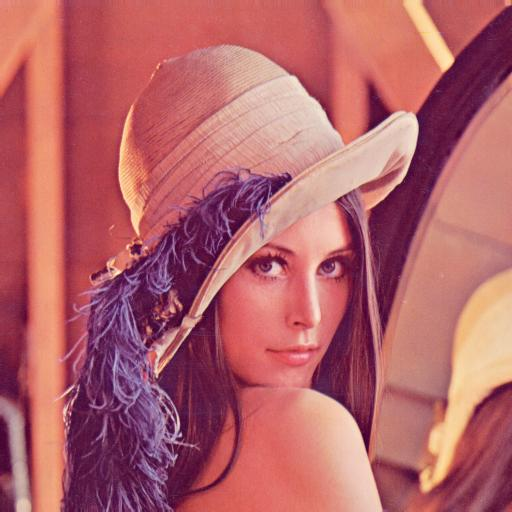
\includegraphics[scale=0.48]{./images/lenacolor.jpg}
    % lenacolor.jpg: 512x512 pixel, 96dpi, 13.55x13.55 cm, bb=0 0 384 384
    \caption{Imagen de Lena. Imagen portadora original.}\label{fig:awesome_image1}
\endminipage\hfill
\minipage[c]{0.5\textwidth}
    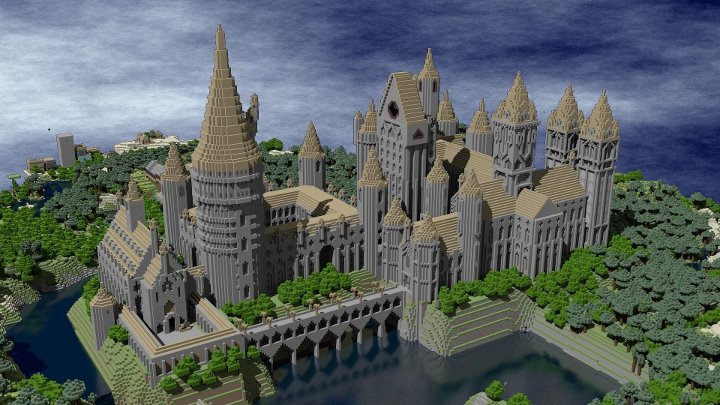
\includegraphics[scale=0.3]{./images/hogwarts.jpg}
    % hogwarts.jpg: 720x405 pixel, 300dpi, 6.10x3.43 cm, bb=0 0 173 97
    \caption{Imagen que se quiere ocultar. Imagen JPG del castillo de Hogwarts en Minecraft.}\label{fig:awesome_image2}
\endminipage\hfill
\end{figure}


\begin{figure}[!htb]
\minipage{0.58\textwidth}    
    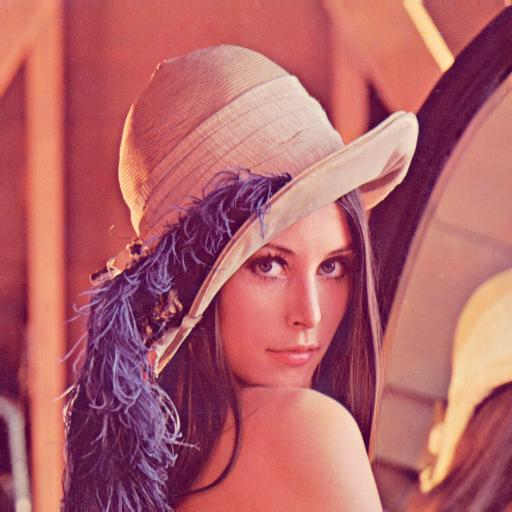
\includegraphics[scale=0.5]{./images/lenacolor-lsb1.jpg}
    % lenacolor-lsb1.jpg: 512x512 pixel, 96dpi, 13.55x13.55 cm, bb=0 0 384 384
    \caption{Resultado de ocultar la imagen \ref{fig:awesome_image2} en \ref{fig:awesome_image1} utilizando LSB1. }\label{fig:awesome_image3}
\endminipage\hfill
\minipage{0.5\textwidth}
    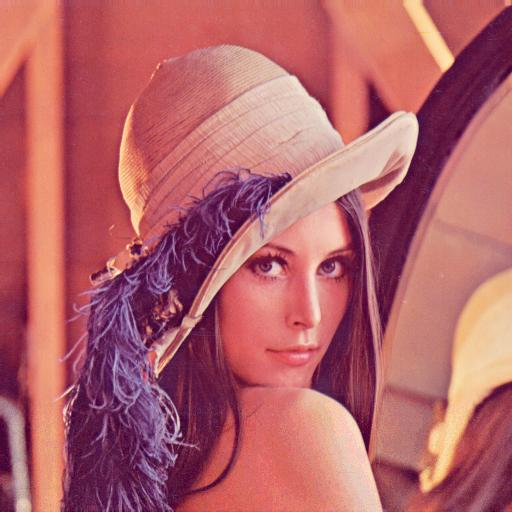
\includegraphics[scale=0.5]{./images/lenacolor-lsb4.jpg}
    % lenacolor-lsb4.jpg: 512x512 pixel, 96dpi, 13.55x13.55 cm, bb=0 0 384 384
    \caption{Resultado de ocultar la imagen \ref{fig:awesome_image2} en \ref{fig:awesome_image1} utilizando LSB4. Se puede observar que comienza a haber un poco de ruido
    apreciable, sobre todo en la parte del hombro.}\label{fig:awesome_image4}
\endminipage\hfill
\end{figure}


\begin{figure}[!htb]
\minipage{0.48\textwidth}
   \includegraphics[scale=0.075]{./images/secretodesusojos1.png}
    % secretodesusojos1.png: 2480x3528 pixel, 96dpi, 65.61x93.33 cm, bb=0 0 1860 2646
  \caption{El secreto de sus ojos. Esteganografiada con el método ``misterioso'' (appendear texto al final del archivo BMP).}\label{fig:awesome_image5}
\endminipage\hfill
\minipage{0.5\textwidth}
   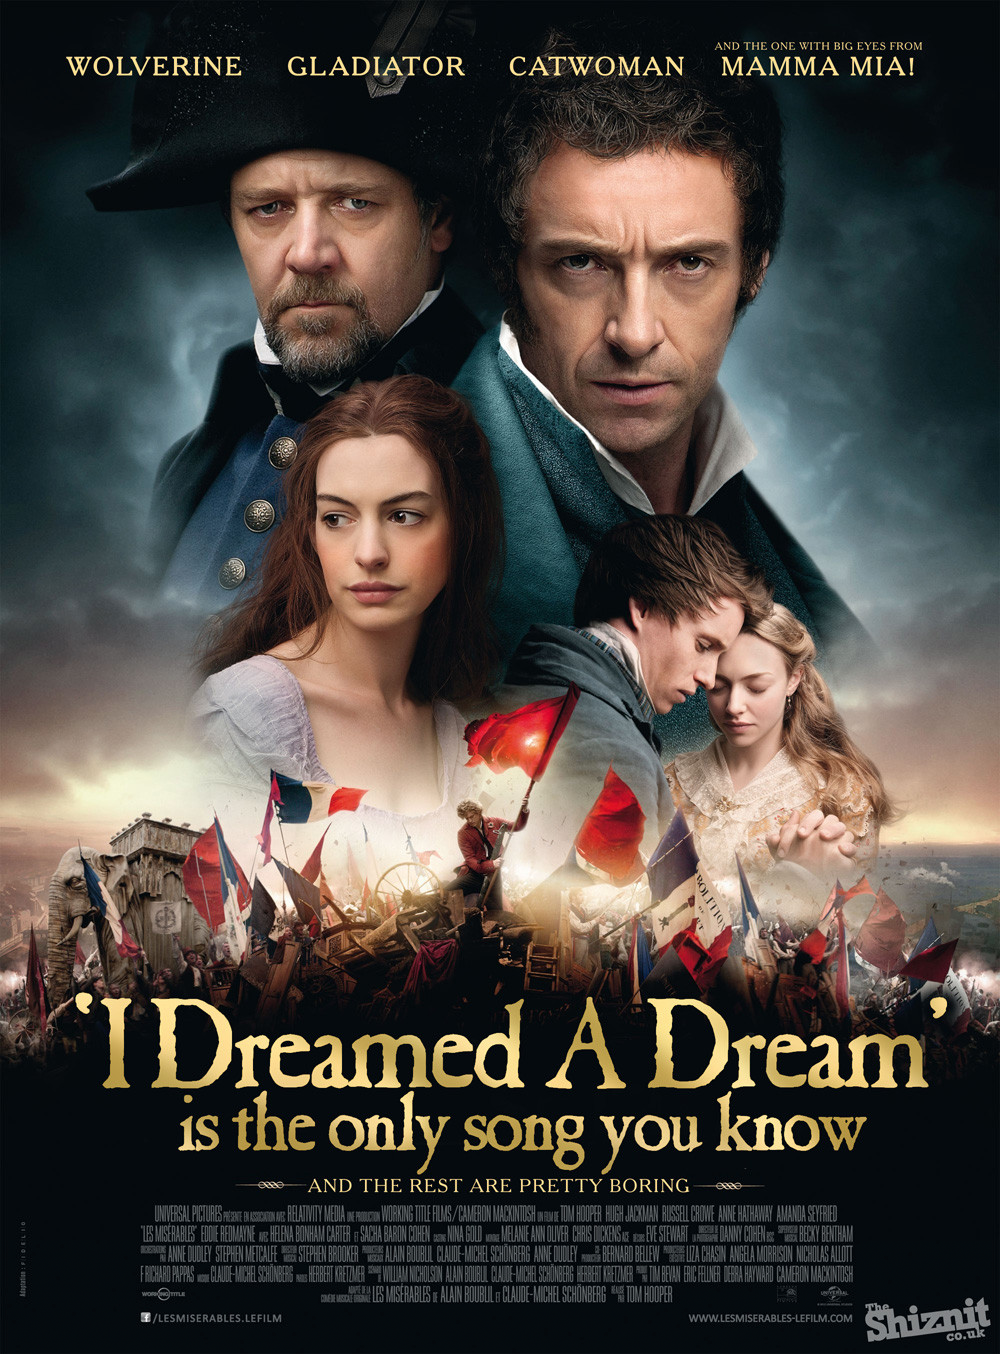
\includegraphics[scale=0.15]{./images/miserables2.png}
    % miserables2.png: 1000x1354 pixel, 72dpi, 35.27x47.76 cm, bb=0 0 1000 1354
  \caption{Los miserables. Esteganografiada con el método LSB1.}\label{fig:awesome_image6}
\endminipage\hfill
\end{figure}

\begin{figure}[!htb]
\minipage{0.48\textwidth}%
  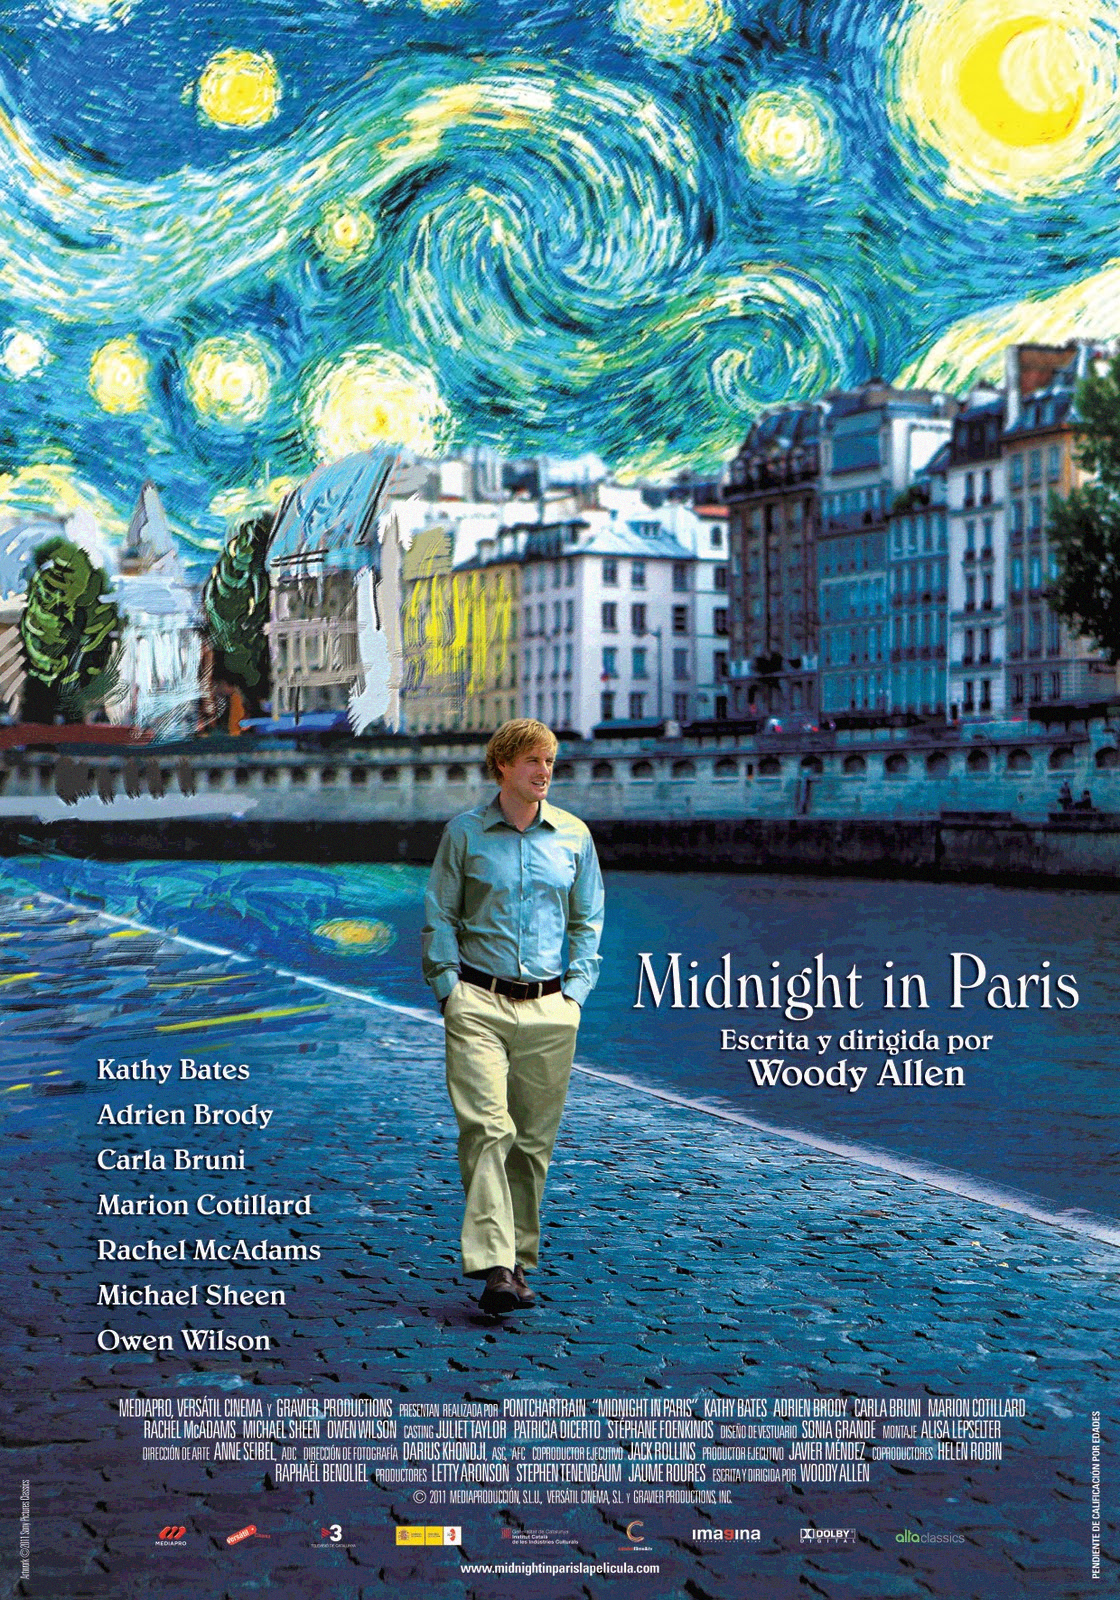
\includegraphics[scale=0.175]{./images/medianocheparis1.png}
  % medianocheparis1.png: 1120x1600 pixel, 96dpi, 29.63x42.33 cm, bb=0 0 840 1200
  \caption{Los miserables. Esteganografiada con el método LSB4 y usando encriptación para el mensaje oculto usando aes de 128 bits en
    modo cbc y con contraseña \textit{bienvenido}.}\label{fig:awesome_image7}
\endminipage
\minipage{0.02\textwidth}%

\endminipage
\minipage{0.5\textwidth}%
   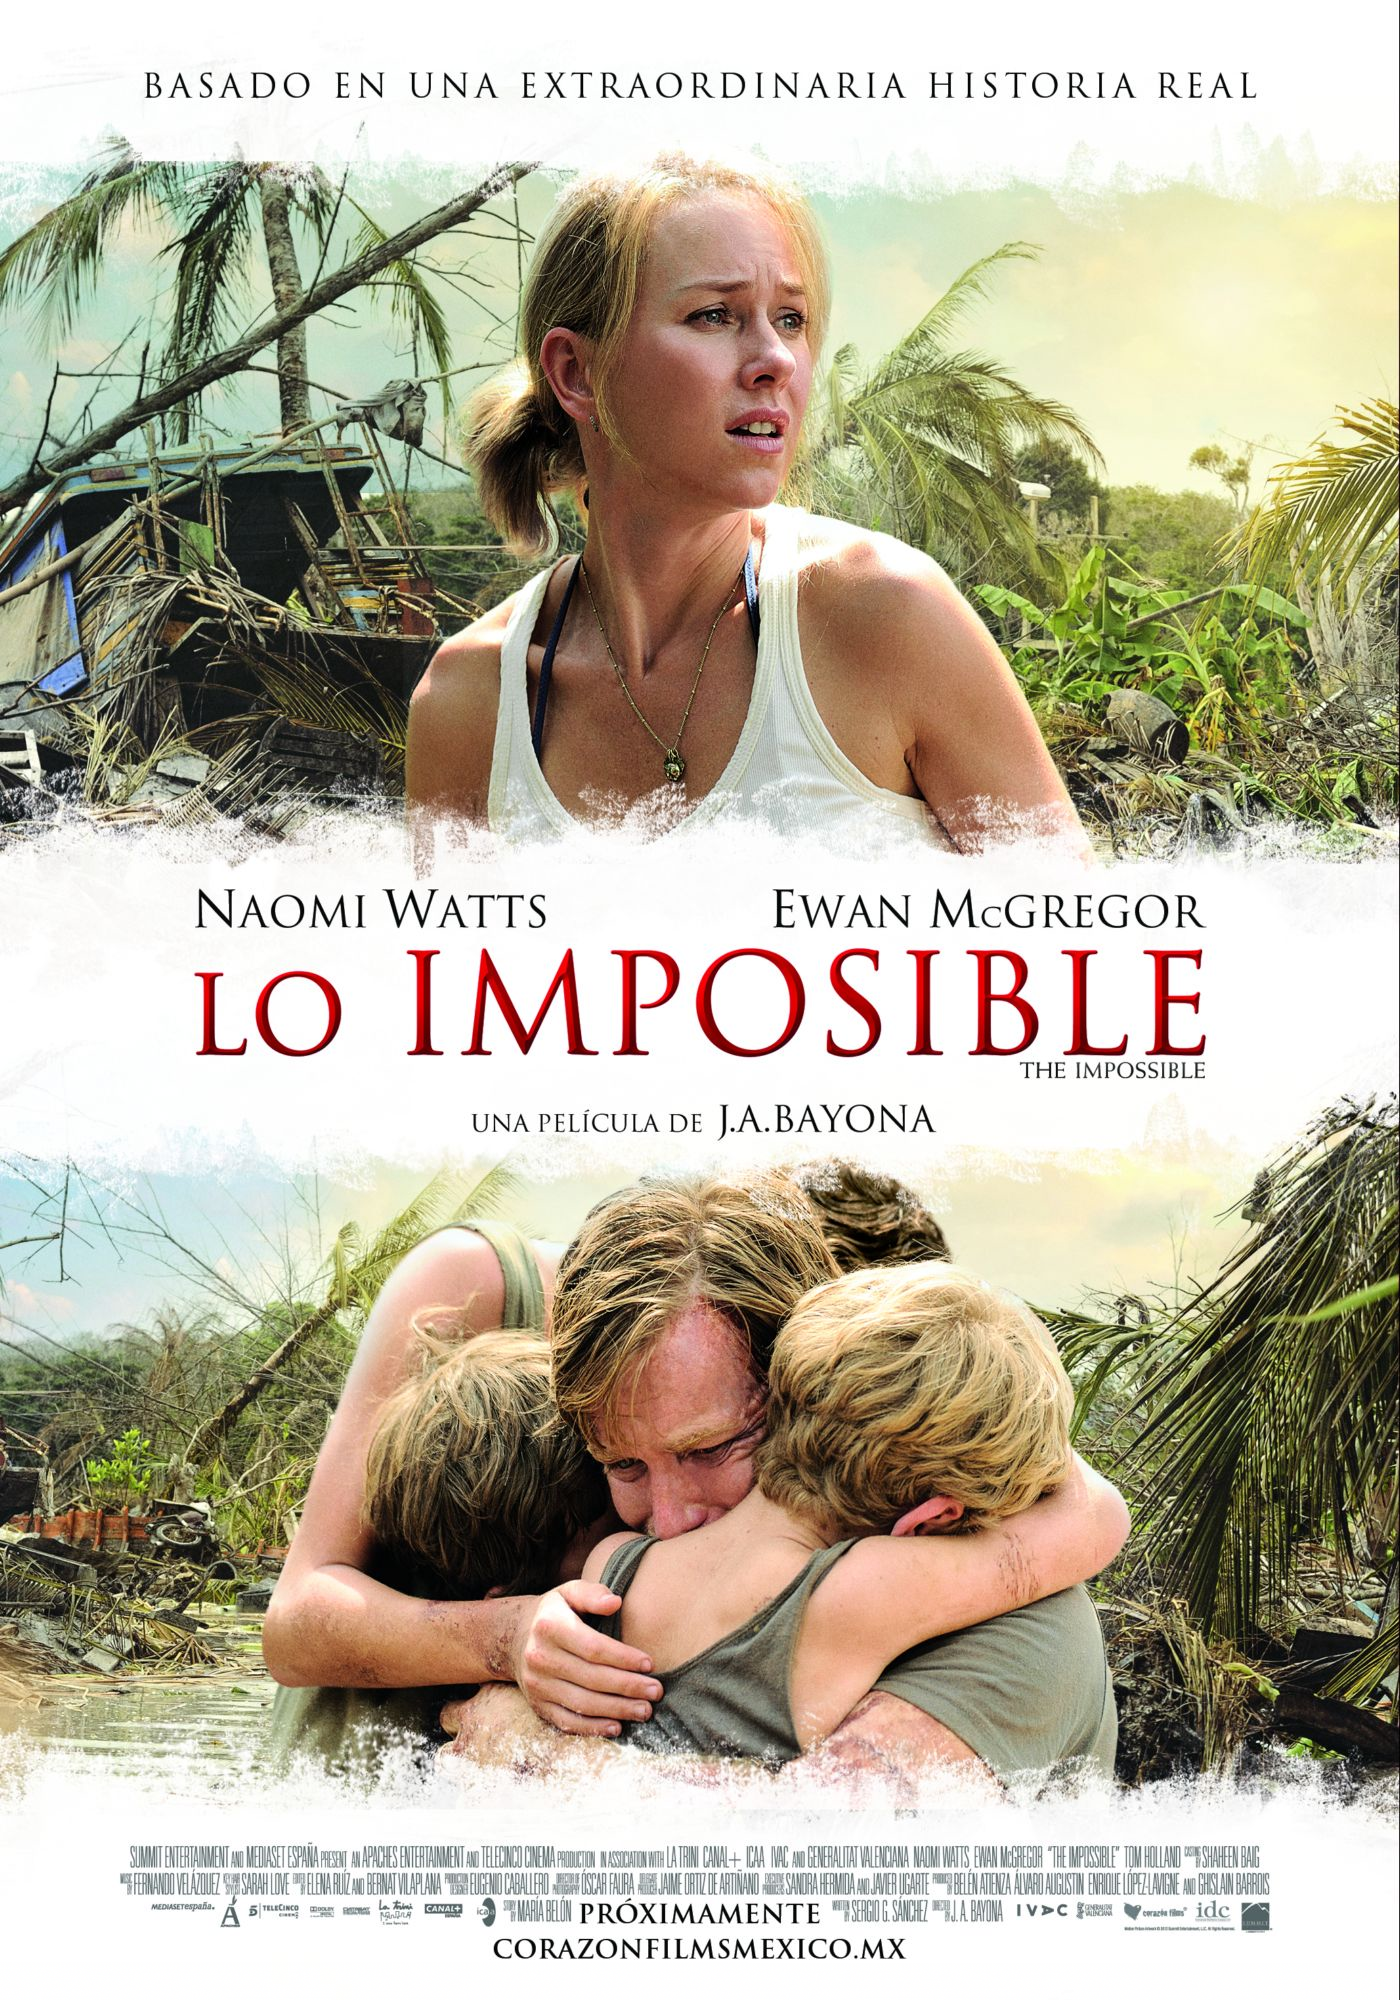
\includegraphics[scale=0.5]{./images/loimposible.png}
    % loimposible.png: 1400x2000 pixel, 300dpi, 11.85x16.93 cm, bb=0 0 336 480
  \caption{Lo imposible. Esteganografiada con el método LSBE.}\label{fig:awesome_image8}
\endminipage
\end{figure}

\clearpage

 
\begin{figure}[!htb]
\begin{center}
\minipage{0.48\textwidth}%
 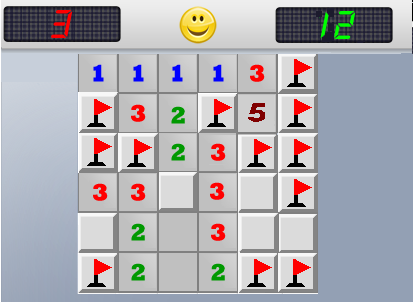
\includegraphics[scale=0.5]{./images/miserables2-out.png}
 % miserables2-out.png: 413x302 pixel, 96dpi, 10.93x7.99 cm, bb=0 0 310 227
  \caption{Imagen PNG. Obtenida utilizando el método LSB1 en la imagen de la figura \ref{fig:awesome_image6}. A la vez, se puede cambiar su extensión por ZIP y 
    descomprimir para obtener un archivo de texto. Además tiene codificado dentro, en forma binaria el algoritmo y el modo de encriptación para desencriptar
    el archivo WMV oculto en la imagen de la figura \ref{fig:awesome_image6}.}\label{fig:awesome_image9}
\endminipage
\end{center}
\end{figure}

\begin{figure}[!htb]
\begin{center}
\minipage{0.48\textwidth}%
 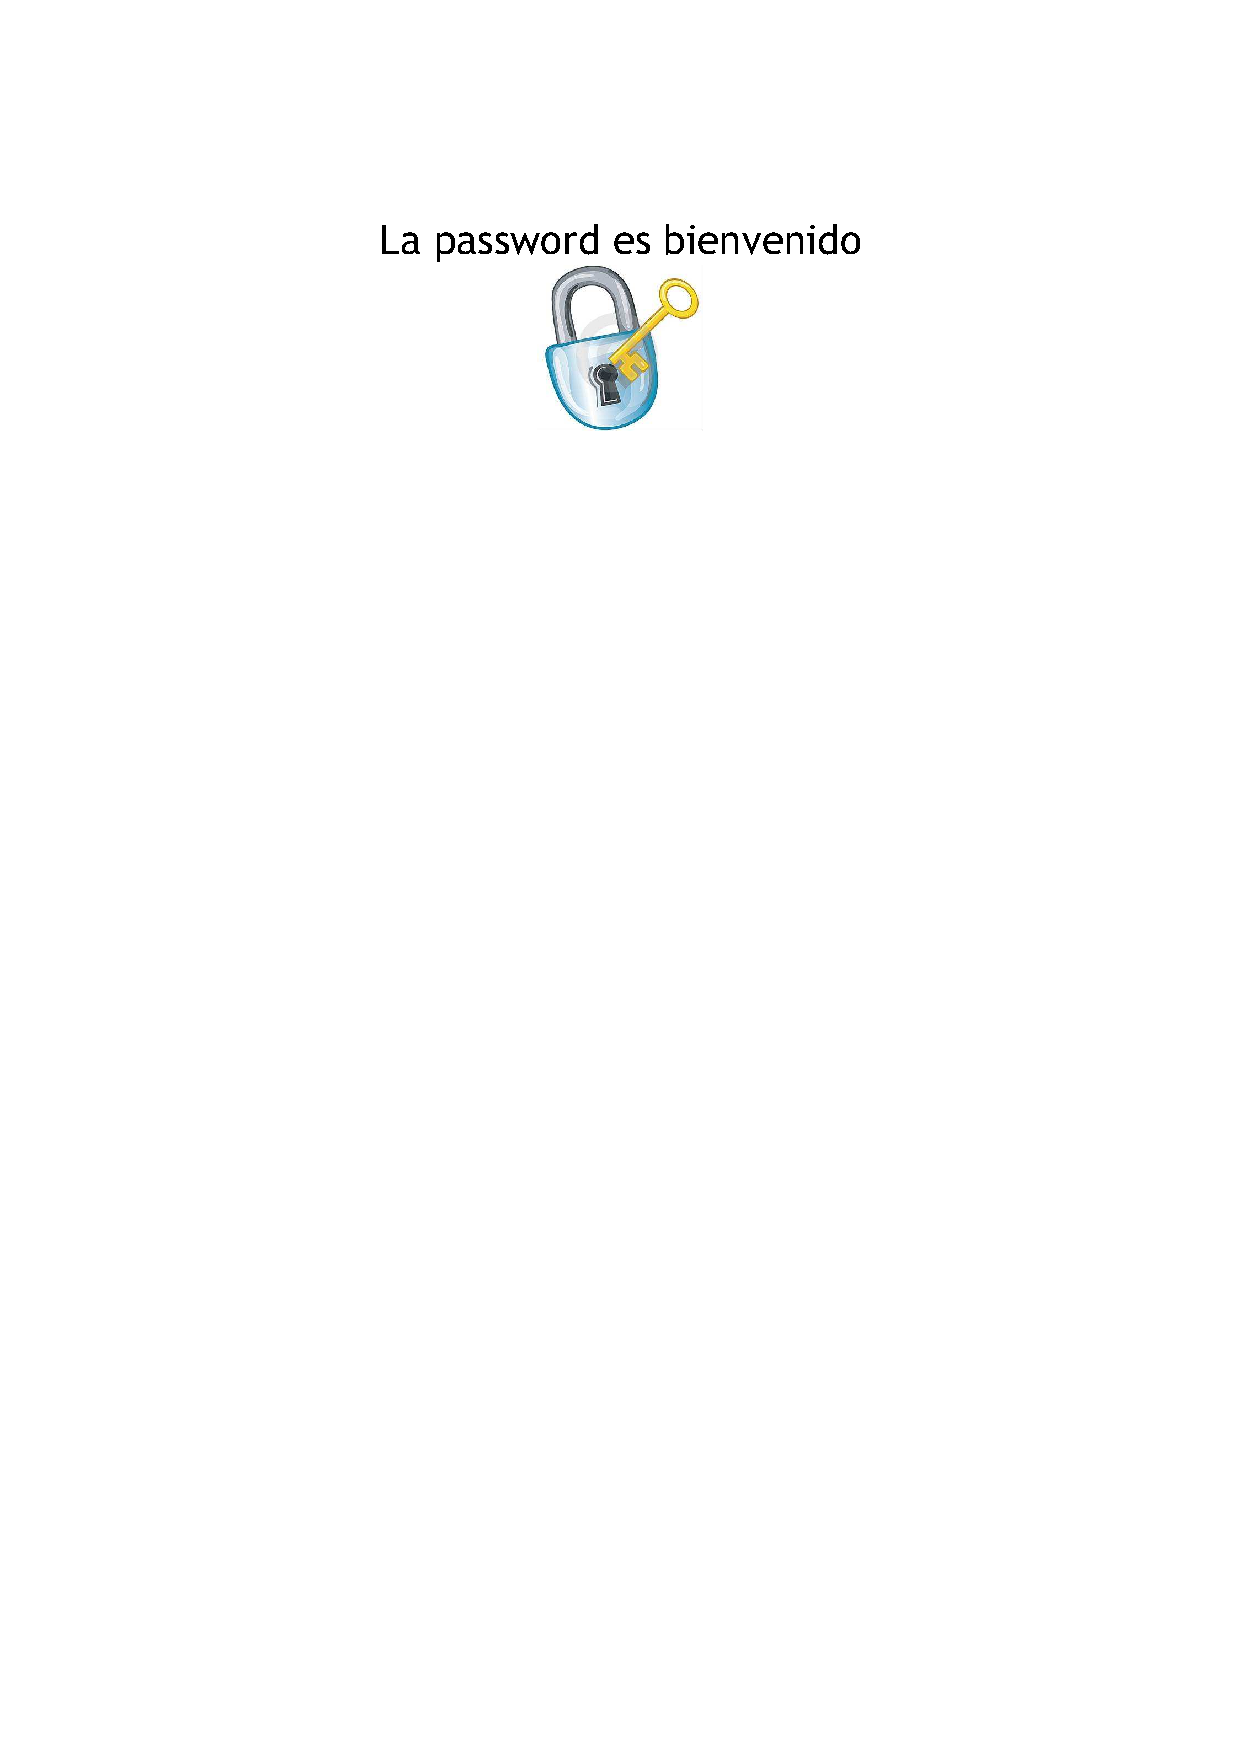
\includegraphics[scale=0.25]{./images/loimposible-out.pdf}
 % loimposible-out.pdf: 595x842 pixel, 72dpi, 20.99x29.70 cm, bb=0 0 595 842
  \caption{Documento PDF. Obtenido a partir de la imagen de la figura \ref{fig:awesome_image8}. Brinda la constraseña para desencriptar el archivo 
    WMV oculto en la imagen de la figura \ref{fig:awesome_image6}.}\label{fig:awesome_image10}
\endminipage
\end{center}
\end{figure}


\end{document}
